%%%%%%%%%%%%%%%%%%%%%%%%%%%%%%%%%%%%%%%%%%%%%%%%%%%%%%%%%%%%%%%%%%%%%%%%
%                                                                      %
%     File: Thesis_Implementation.tex                                  %
%     Tex Master: Thesis.tex                                           %
%                                                                      %
%     Author: Andre C. Marta                                           %
%     Last modified :  2 Jul 2015                                      %
%                                                                      %
%%%%%%%%%%%%%%%%%%%%%%%%%%%%%%%%%%%%%%%%%%%%%%%%%%%%%%%%%%%%%%%%%%%%%%%%

\chapter{Implementation}
\label{chapter:implementation}
\iffalse
Because the stock price depends on a Brownian motion process, it follows that it is not differentiable. For this reason, it's impossible to exactly simulate such a process. An approximation is possible, however, using discrete jumps of length $\Delta t$ and using the Brownian motion property $W(t)\sim \sqrt{t}N(0,1)$~\cite{Mikosch}, with $N(0,1)$ being a normal distribution with 0 expected value and 1 variance.
We can then simply discretize eq. \eqref{BS} into
\begin{equation}
S(t+\Delta t)=S(t)+rS(t)\Delta t+\sqrt{\Delta t}\sigma S(t)N(0,1),
\end{equation}
\noindent where $\Delta t$ corresponds to a given time step. An example of this discretization is illustrated in \autoref{fig:GBM} with the realization of three sample paths.

\begin{figure}[H]
    \centering
      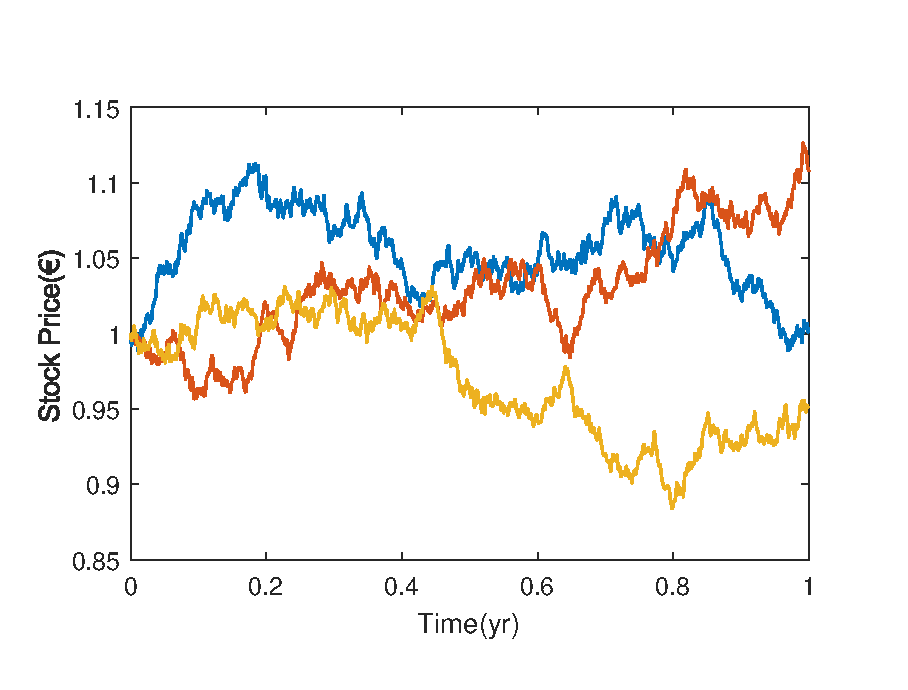
\includegraphics[width=0.9\columnwidth]{GBM.eps}
      \caption{Example of three GBM processes, using the parameters $r=\SI{0.06}{\per\year}$, $\sigma=0.05$, $S(0)=\SI{1}[\EUR]{}$ and time steps $\Delta t=10^{-3}\SI{}{\year}$.}\label{fig:GBM}
    \end{figure}
    
By simulating a large number of paths, some underlying tendencies might become apparent, which will prove useful in option pricing.


 American options, however, pose a much greater challenge.  Unlike European options, no analytic pricing model currently exists for this type of derivatives. Several numerical models have been proposed in the past in an attempt to solve this problem~\cite{Wilmott1,Hull}, such as the Longstaff-Schwartz algorithm~\citep{Longstaff}, which we shall approach in later sections of the present thesis.
\fi
Insert your chapter material here...

%%%%%%%%%%%%%%%%%%%%%%%%%%%%%%%%%%%%%%%%%%%%%%%%%%%%%%%%%%%%%%%%%%%%%%%%
\section{Numerical Model}
\label{section:model}

Description of the numerical implementation of the models explained in Chapter~\ref{chapter:background}...


%%%%%%%%%%%%%%%%%%%%%%%%%%%%%%%%%%%%%%%%%%%%%%%%%%%%%%%%%%%%%%%%%%%%%%%%
\section{Verification and Validation}
\label{section:verification}

Basic test cases to compare the implemented model against other numerical tools (verification) and experimental data (validation)...

